\chapter{Apresentação do Sistema}

\section{Tecnologias a serem usadas no Frontend}

O aplicativo foi desenvolvido em \textbf{React Native 0.74} com o runtime do \textbf{Expo SDK 51}, utilizando o modelo de componentes funcionais e API de Hooks do React. As principais bibliotecas adotadas são:

\begin{itemize}
    \item \textbf{@react-navigation/native + createNativeStackNavigator:} Controle da hierarquia de telas (pilhas pública e privada) e navegação programática entre rotas.
    \item \textbf{Redux Toolkit:} Gerência global de estado com dois \textit{slices}: \texttt{token.js} (sessão JWT) e \texttt{snackBar.js} (notificações de feedback global).
    \item \textbf{expo-secure-store:} Armazenamento criptografado do token JWT no cofre nativo do sistema operacional (\textit{Keychain} no iOS, \textit{KeyStore} no Android).
    \item \textbf{expo-camera (CameraView):} Captura de câmera nativa para leitura de QR Code com validação por \texttt{boundingBox}.
    \item \textbf{react-native-gesture-handler (Swipeable):} Gestos de deslizamento horizontal em cards da lista de eventos e convidados.
    \item \textbf{react-native-draggable-flatlist:} Lista com suporte a reordenação por arrastar-e-soltar (\textit{Drag 'n Drop}) a 60fps.
    \item \textbf{react-native-paper:} Componentes visuais baseados em \textit{Material Design} (inputs, dialogs, FAB).
    \item \textbf{expo-font (Poppins):} Família tipográfica carregada assincronamente na inicialização (Regular, Bold, Black, ExtraBold).
    \item \textbf{expo-image-picker:} Seleção e compressão de fotos da galeria ou câmera.
    \item \textbf{expo-document-picker + expo-file-system:} Seleção de arquivos \texttt{.docx} e leitura em Base64 para upload do template de certificado.
    \item \textbf{react-native-webview:} Renderização do PDF de pré-visualização do certificado diretamente no aplicativo.
    \item \textbf{Axios:} Cliente HTTP com interceptors que injetam automaticamente o cabeçalho \texttt{Authorization: Bearer \{token\}} em todas as requisições autenticadas.
    \item \textbf{@fortawesome/react-native-fontawesome:} Ícones vetoriais (lixeira, chevron, check, refresh, etc.).
    \item \textbf{date-fns:} Utilitário de formatação de datas no frontend (ex: \texttt{format(date, "dd/MM/yyyy")}).
\end{itemize}

\section{Projeto das Interfaces}

A seguir são apresentadas as interfaces do sistema Certify, com descrições baseadas na análise direta dos arquivos-fonte de cada tela. As imagens deverão ser substituídas pelas capturas de tela reais do aplicativo durante a etapa de finalização do documento.

% ───────────────────
\begin{figure}[H]
    \centering
    \caption{Tela de Login (\texttt{login.js})}
    \vspace{0.4cm}
    
\includegraphics[width=0.45\textwidth,keepaspectratio]{imagens/app/login.jpg}
    \vspace{0.4cm}
    \end{figure}

A tela de Login é o ponto de entrada seguro para a área restrita do organizador. A interface realiza validações visuais instantâneas nos campos inseridos, fornecendo feedback imediato caso o formato do e-mail ou senha esteja incorreto. Após a autenticação bem-sucedida, a sessão é protegida no dispositivo e o usuário é redirecionado de forma fluida para o painel principal.


% ───────────────────
\begin{figure}[H]
    \centering
    \caption{Tela Inicial — Lista de Eventos (\texttt{home.js})}
    \vspace{0.4cm}
    
\includegraphics[width=0.45\textwidth,keepaspectratio]{imagens/app/list_events.jpg}
    \vspace{0.4cm}
    \end{figure}

A tela inicial lista todos os eventos do organizador autenticado, exibindo de forma clara o status atual de cada um. Os filtros rápidos na parte superior permitem alternar entre eventos ativos e passados de maneira instantânea. Para facilitar a gestão, gestos nativos de deslizamento lateral (\textit{swipe}) em cada cartão revelam opções de ação rápida, como a exclusão de um evento.

% ───────────────────
\begin{figure}[H]
    \centering
    \caption{Confirmação de Exclusão de Evento}
    \vspace{0.4cm}
    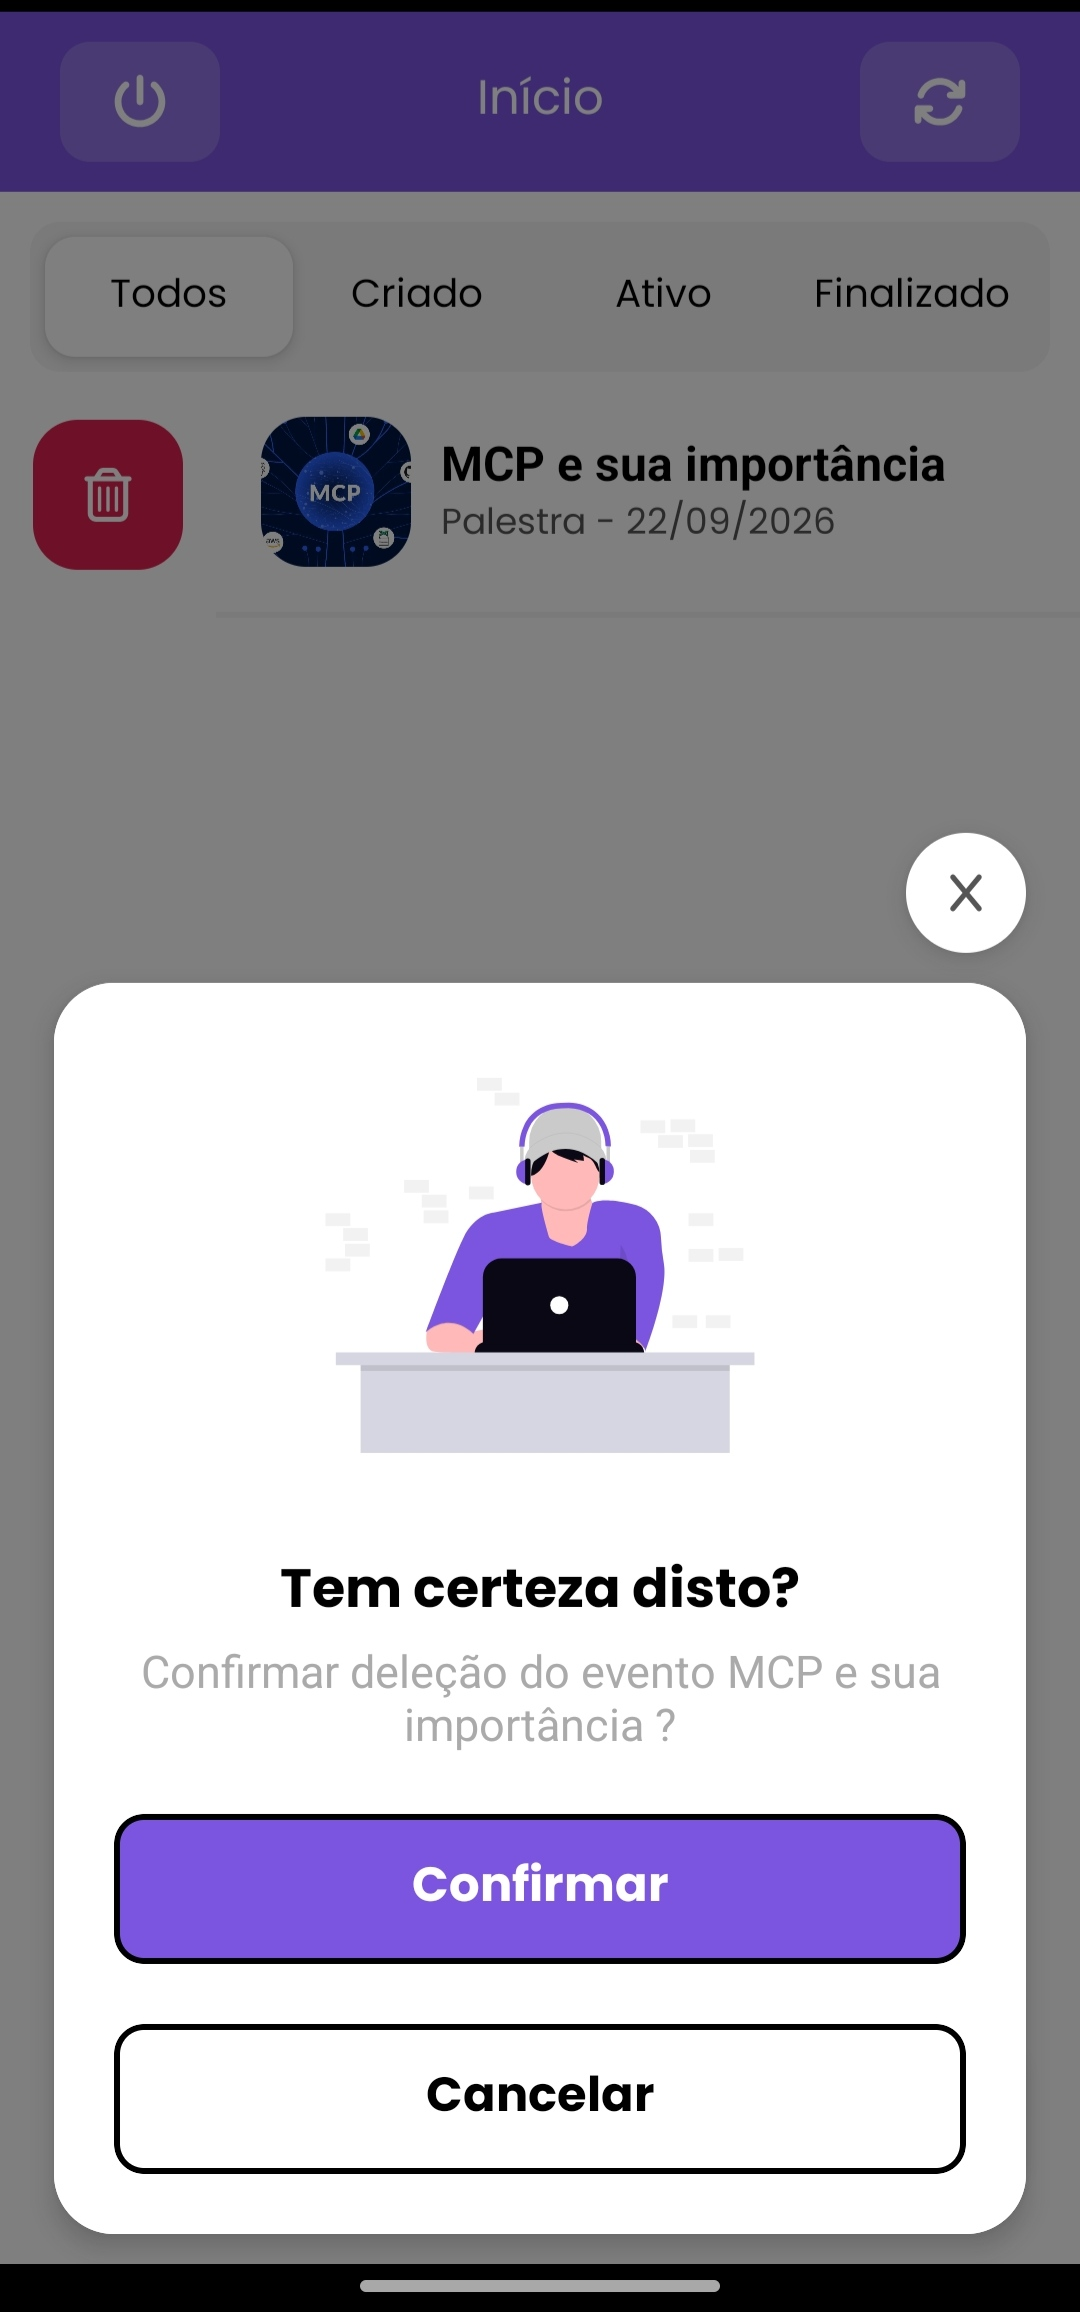
\includegraphics[width=0.45\textwidth,keepaspectratio]{imagens/app/event_confirm_delete.jpg}
    \vspace{0.4cm}
    \end{figure}

Sempre que uma ação destrutiva é solicitada, o sistema exibe alertas modais de confirmação claros para prevenir perdas acidentais de dados.

% ───────────────────
\begin{figure}[H]
    \centering
    \caption{Criação de Novo Evento (\texttt{newEvent.js})}
    \vspace{0.4cm}
    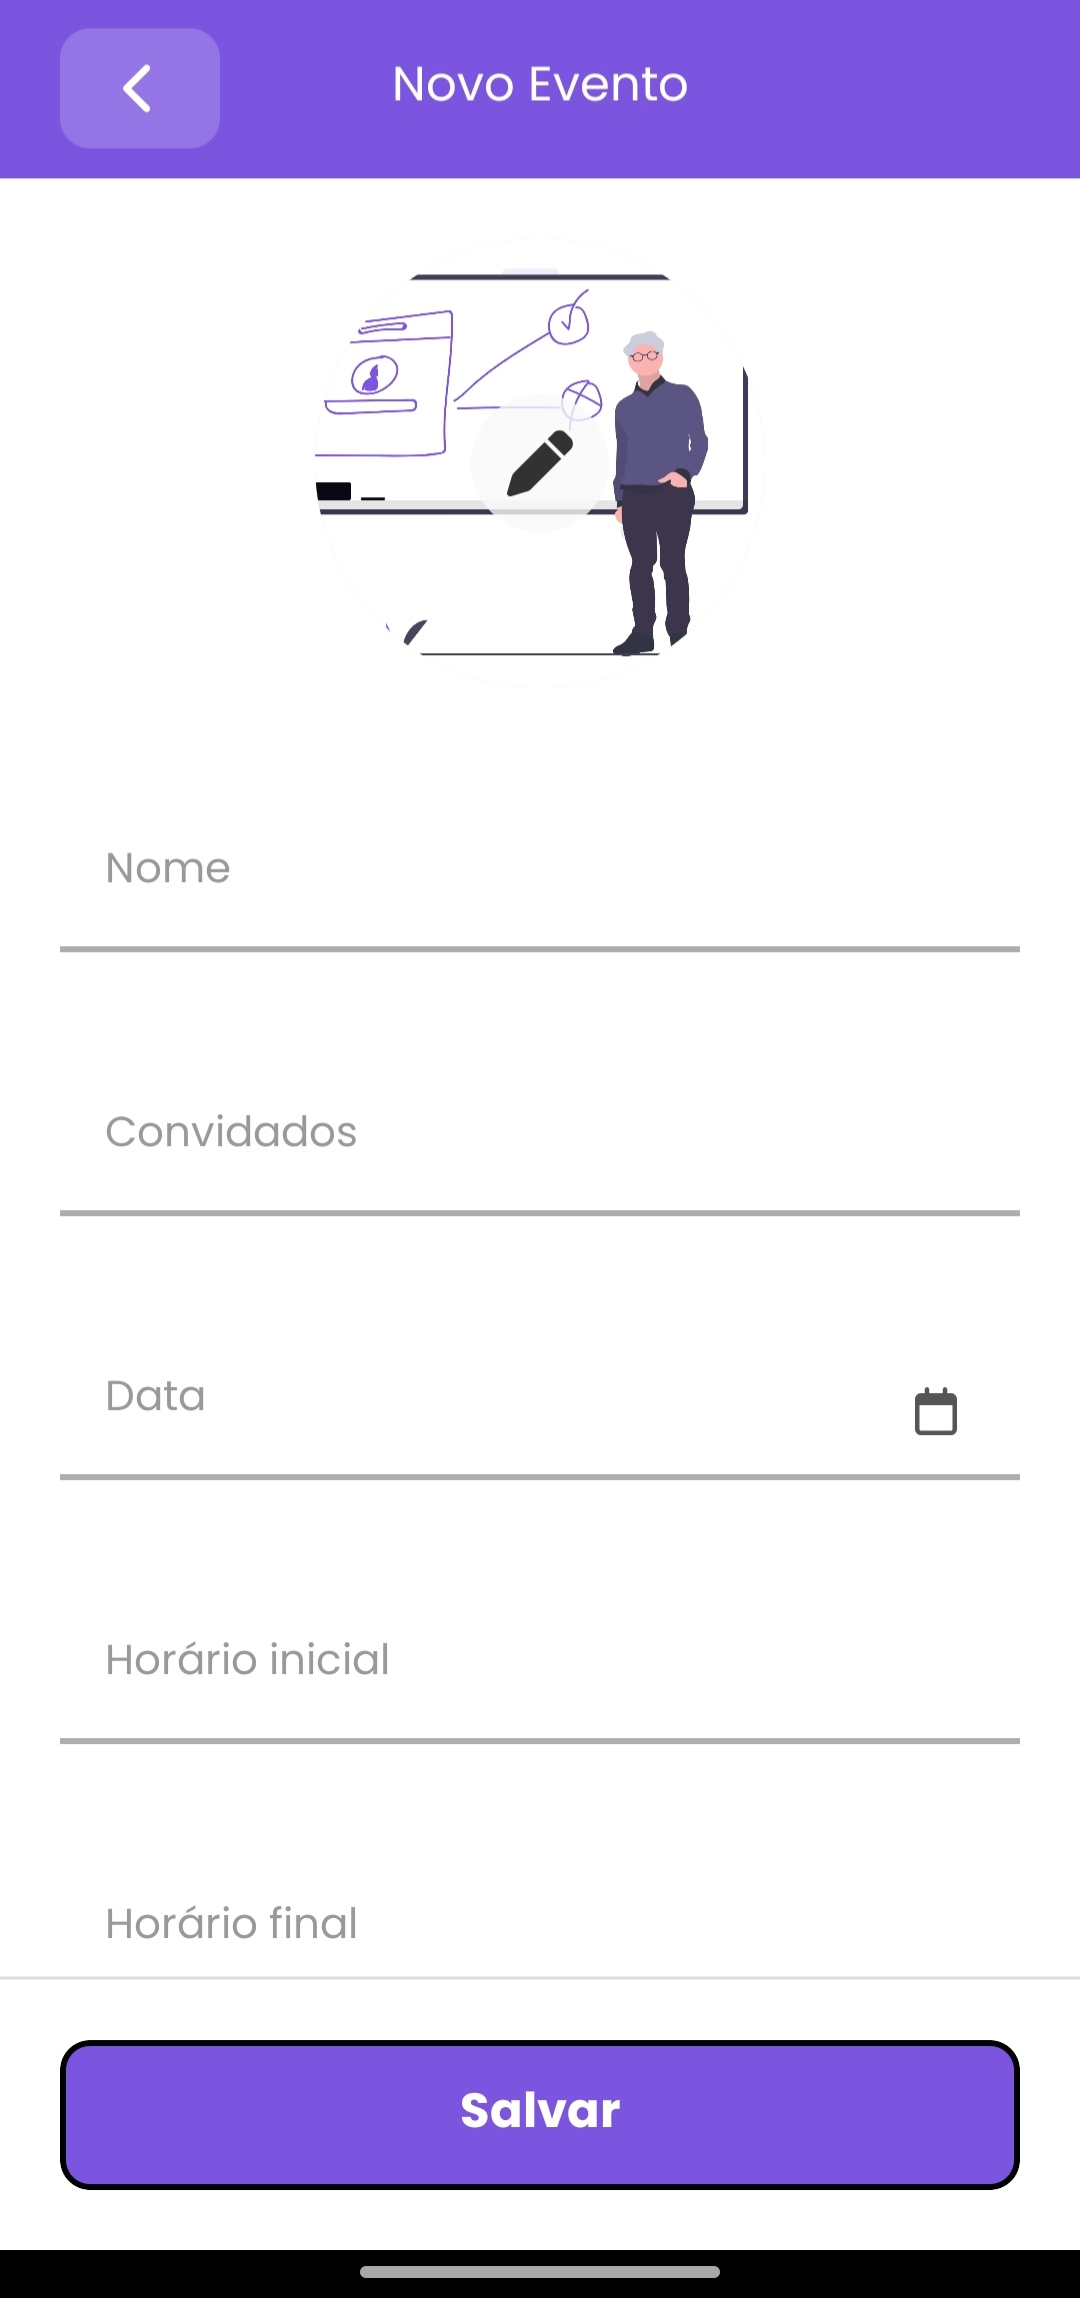
\includegraphics[width=0.45\textwidth,keepaspectratio]{imagens/app/new_event.jpg}
    \vspace{0.4cm}
    \end{figure}

O formulário de criação de evento guia o organizador no preenchimento dos detalhes principais, adotando componentes intuitivos de data, hora e seleções simplificadas para evitar fricção na configuração inicial.

% ───────────────────
\begin{figure}[H]
    \centering
    \caption{Aba de Informações do Evento (\texttt{eventTab.js})}
    \vspace{0.4cm}
    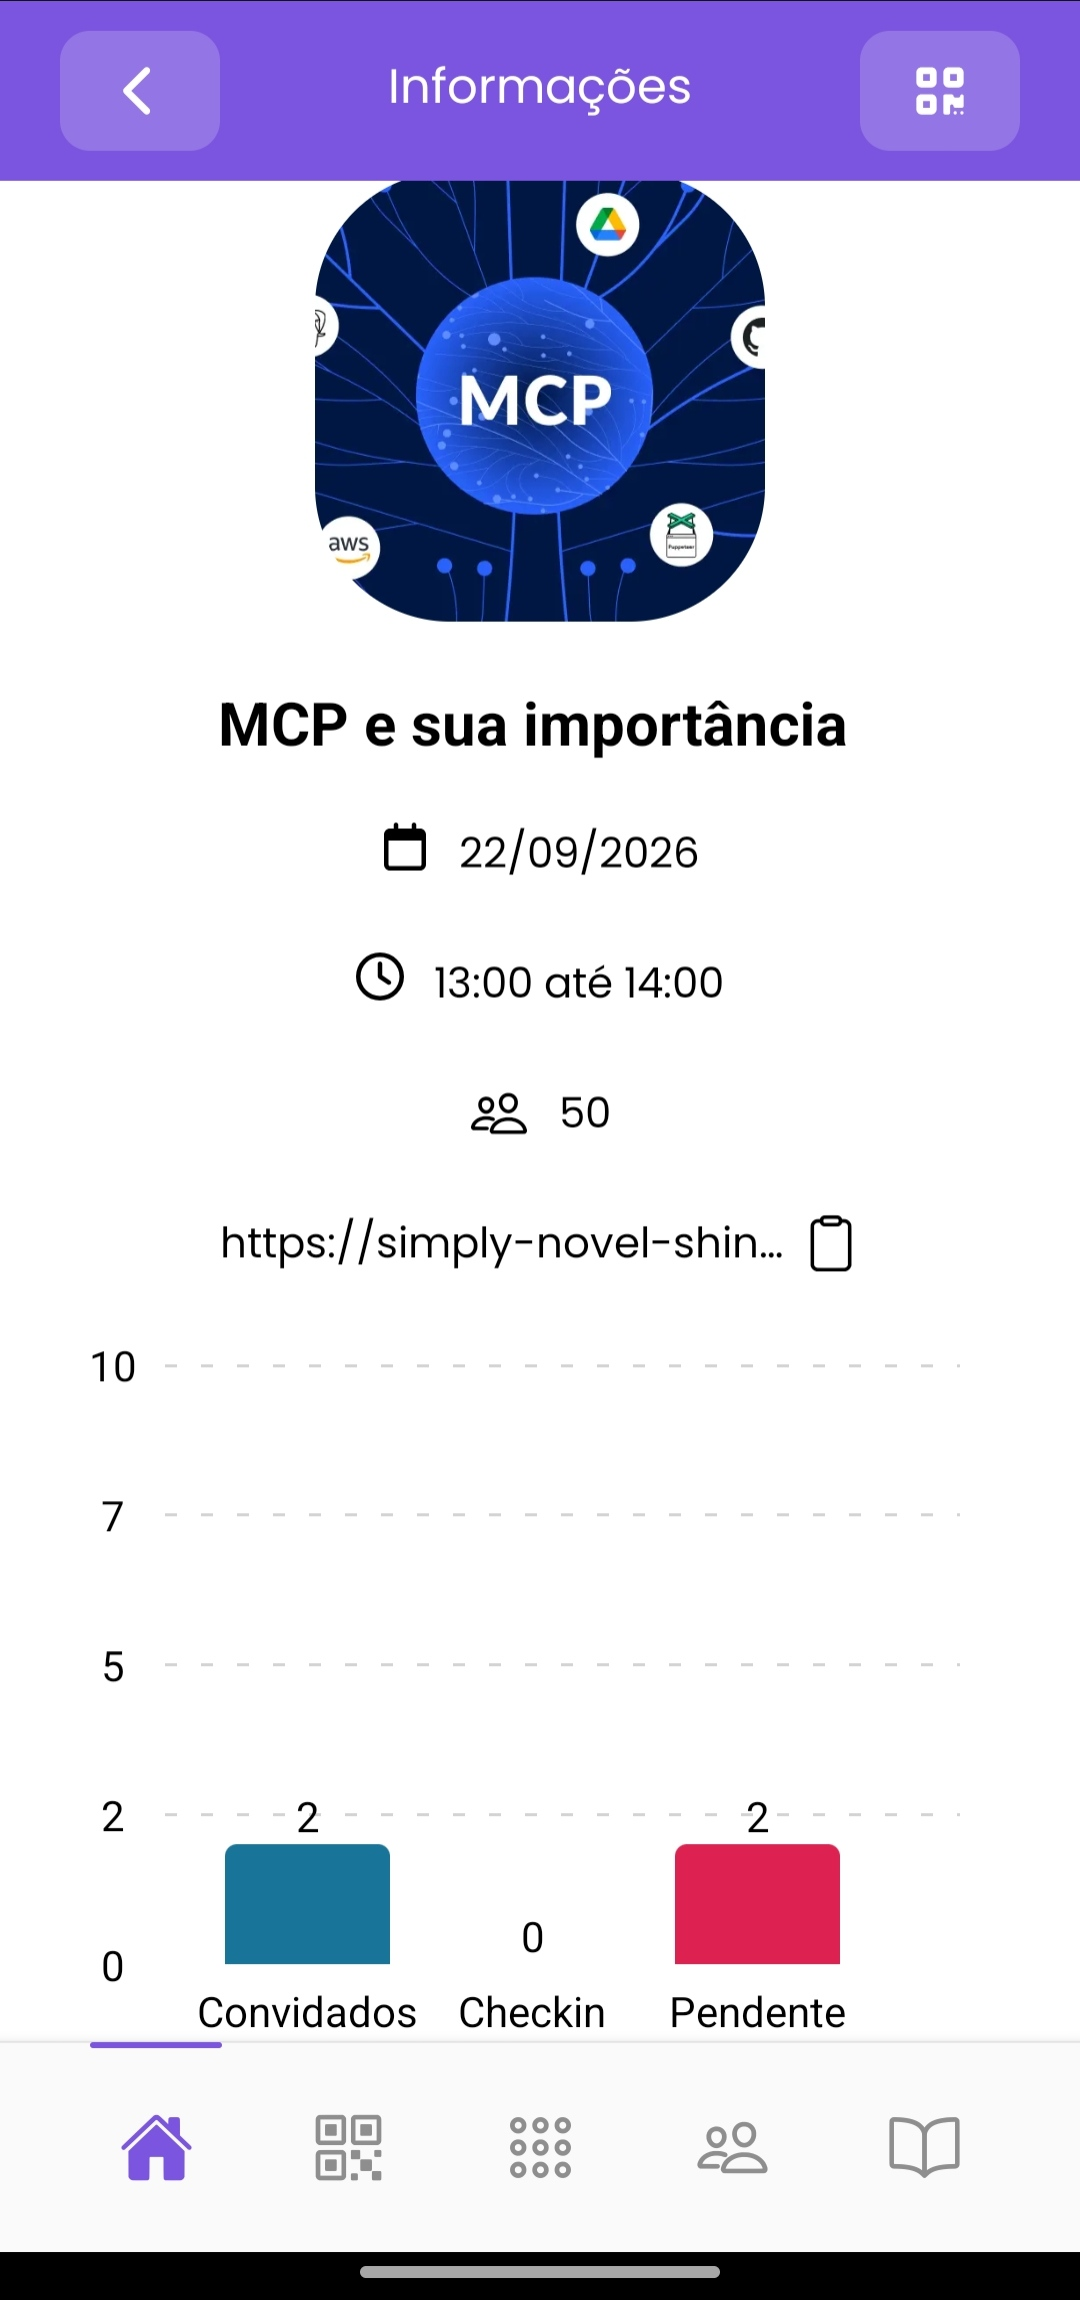
\includegraphics[width=0.45\textwidth,keepaspectratio]{imagens/app/event_dashboard.jpg}
    \vspace{0.4cm}
    \end{figure}

O painel de controle do evento concentra os dados gerais, métricas de comparecimento e as principais ações organizacionais. Um dos destaques de usabilidade é o controle centralizado do status de inscrições e check-ins, que o organizador pode ativar ou suspender rapidamente com um toque.

% ───────────────────
\begin{figure}[H]
    \centering
    \caption{Exibição do QR Code do Evento}
    \vspace{0.4cm}
    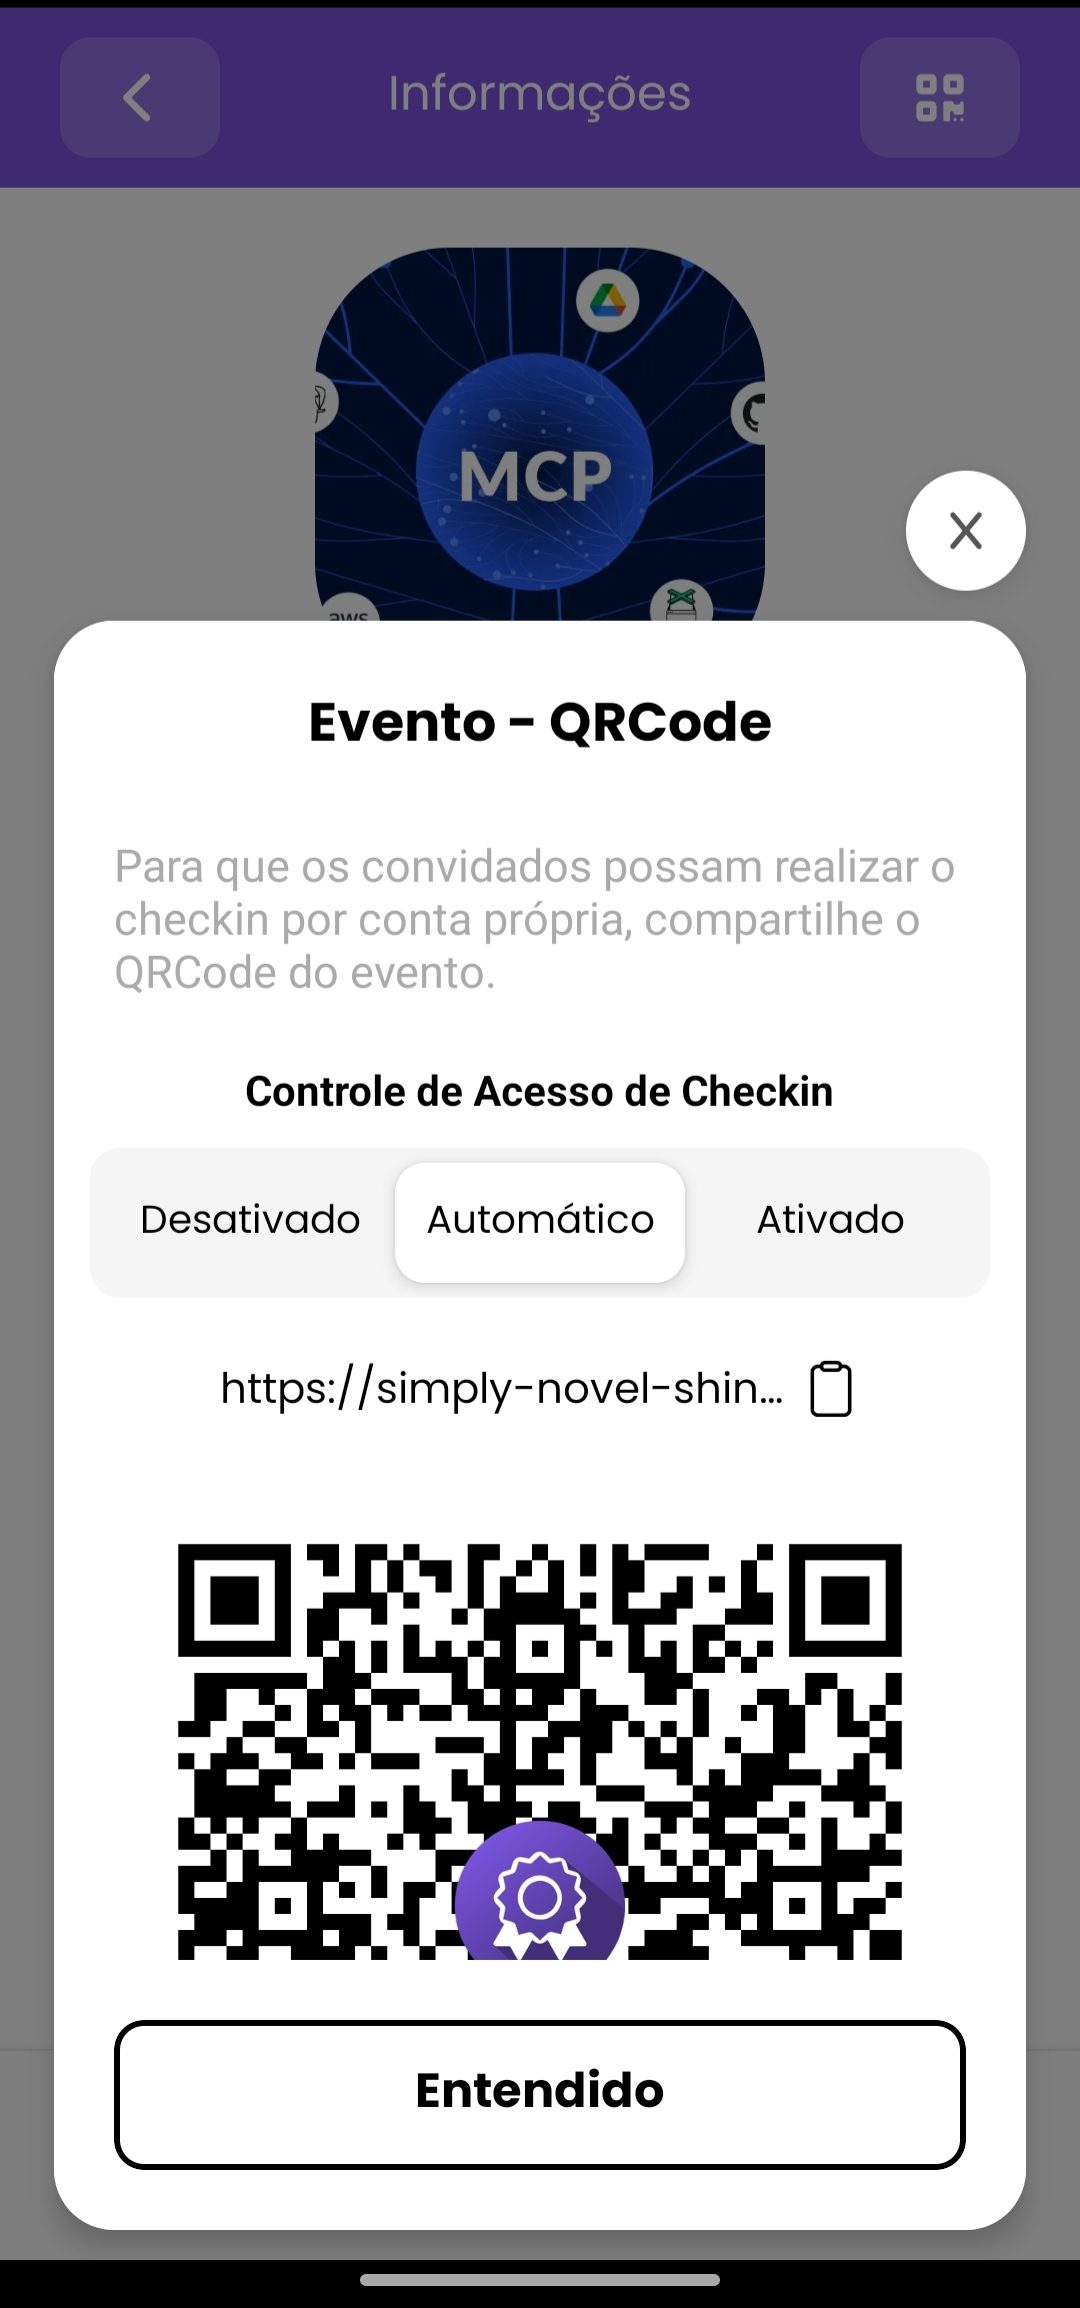
\includegraphics[width=0.45\textwidth,keepaspectratio]{imagens/app/event_checkin_qrcode.jpg}
    \vspace{0.4cm}
    \end{figure}

A partir do painel, o organizador pode exibir rapidamente o QR Code oficial do evento em tela cheia. Essa facilidade permite o uso do próprio aparelho como uma central móvel para direcionar convidados ou habilitar totens de autoatendimento.

% ───────────────────
\begin{figure}[H]
    \centering
    \caption{Leitor de QR Code (\texttt{eventScanner.js})}
    \vspace{0.4cm}
    
\includegraphics[width=0.45\textwidth,keepaspectratio]{imagens/app/qrcode_scanner.jpg}
    \vspace{0.4cm}
    \end{figure}

A tela de scanner maximiza a área útil do visor ao remover o cabeçalho padrão, oferecendo uma experiência de leitura imersiva e direta. Guias visuais animadas nos cantos da tela foram implementadas para orientar o foco do usuário. Além disso, para evitar leituras acidentais ou incorretas de códigos próximos, o sistema valida a posição espacial do código QR detectado, processando o check-in apenas se o código estiver perfeitamente enquadrado dentro dos limites do quadro de mira na tela.

% ───────────────────
\begin{figure}[H]
    \centering
    \caption{Gerenciamento de Campos Dinâmicos (\texttt{eventFields.js})}
    \vspace{0.4cm}
    
\includegraphics[width=0.45\textwidth,keepaspectratio]{imagens/app/list_dynamic_fields.jpg}
    \vspace{0.4cm}
    \end{figure}

A tela de gerenciamento de campos permite estruturar os formulários de inscrição conforme a necessidade do evento. Para garantir uma ordenação intuitiva, foi adotada uma interface interativa de arrastar-e-soltar (\textit{drag-and-drop}), onde o organizador organiza fisicamente a sequência visual dos campos.

% ───────────────────
\begin{figure}[H]
    \centering
    \caption{Campos Dinâmicos — Estado Vazio}
    \vspace{0.4cm}
    
\includegraphics[width=0.45\textwidth,keepaspectratio]{imagens/app/empty_dynamic_fields.jpg}
    \vspace{0.4cm}
    \end{figure}

Quando nenhum campo foi adicionado ainda, o sistema exibe telas de estado vazio (\textit{empty states}) amigáveis e informativas, orientando o usuário sobre o propósito daquela tela e incentivando-o a iniciar a configuração.

% ───────────────────
\begin{figure}[H]
    \centering
    \caption{Criação de Novo Campo Dinâmico (\texttt{newField.js})}
    \vspace{0.4cm}
    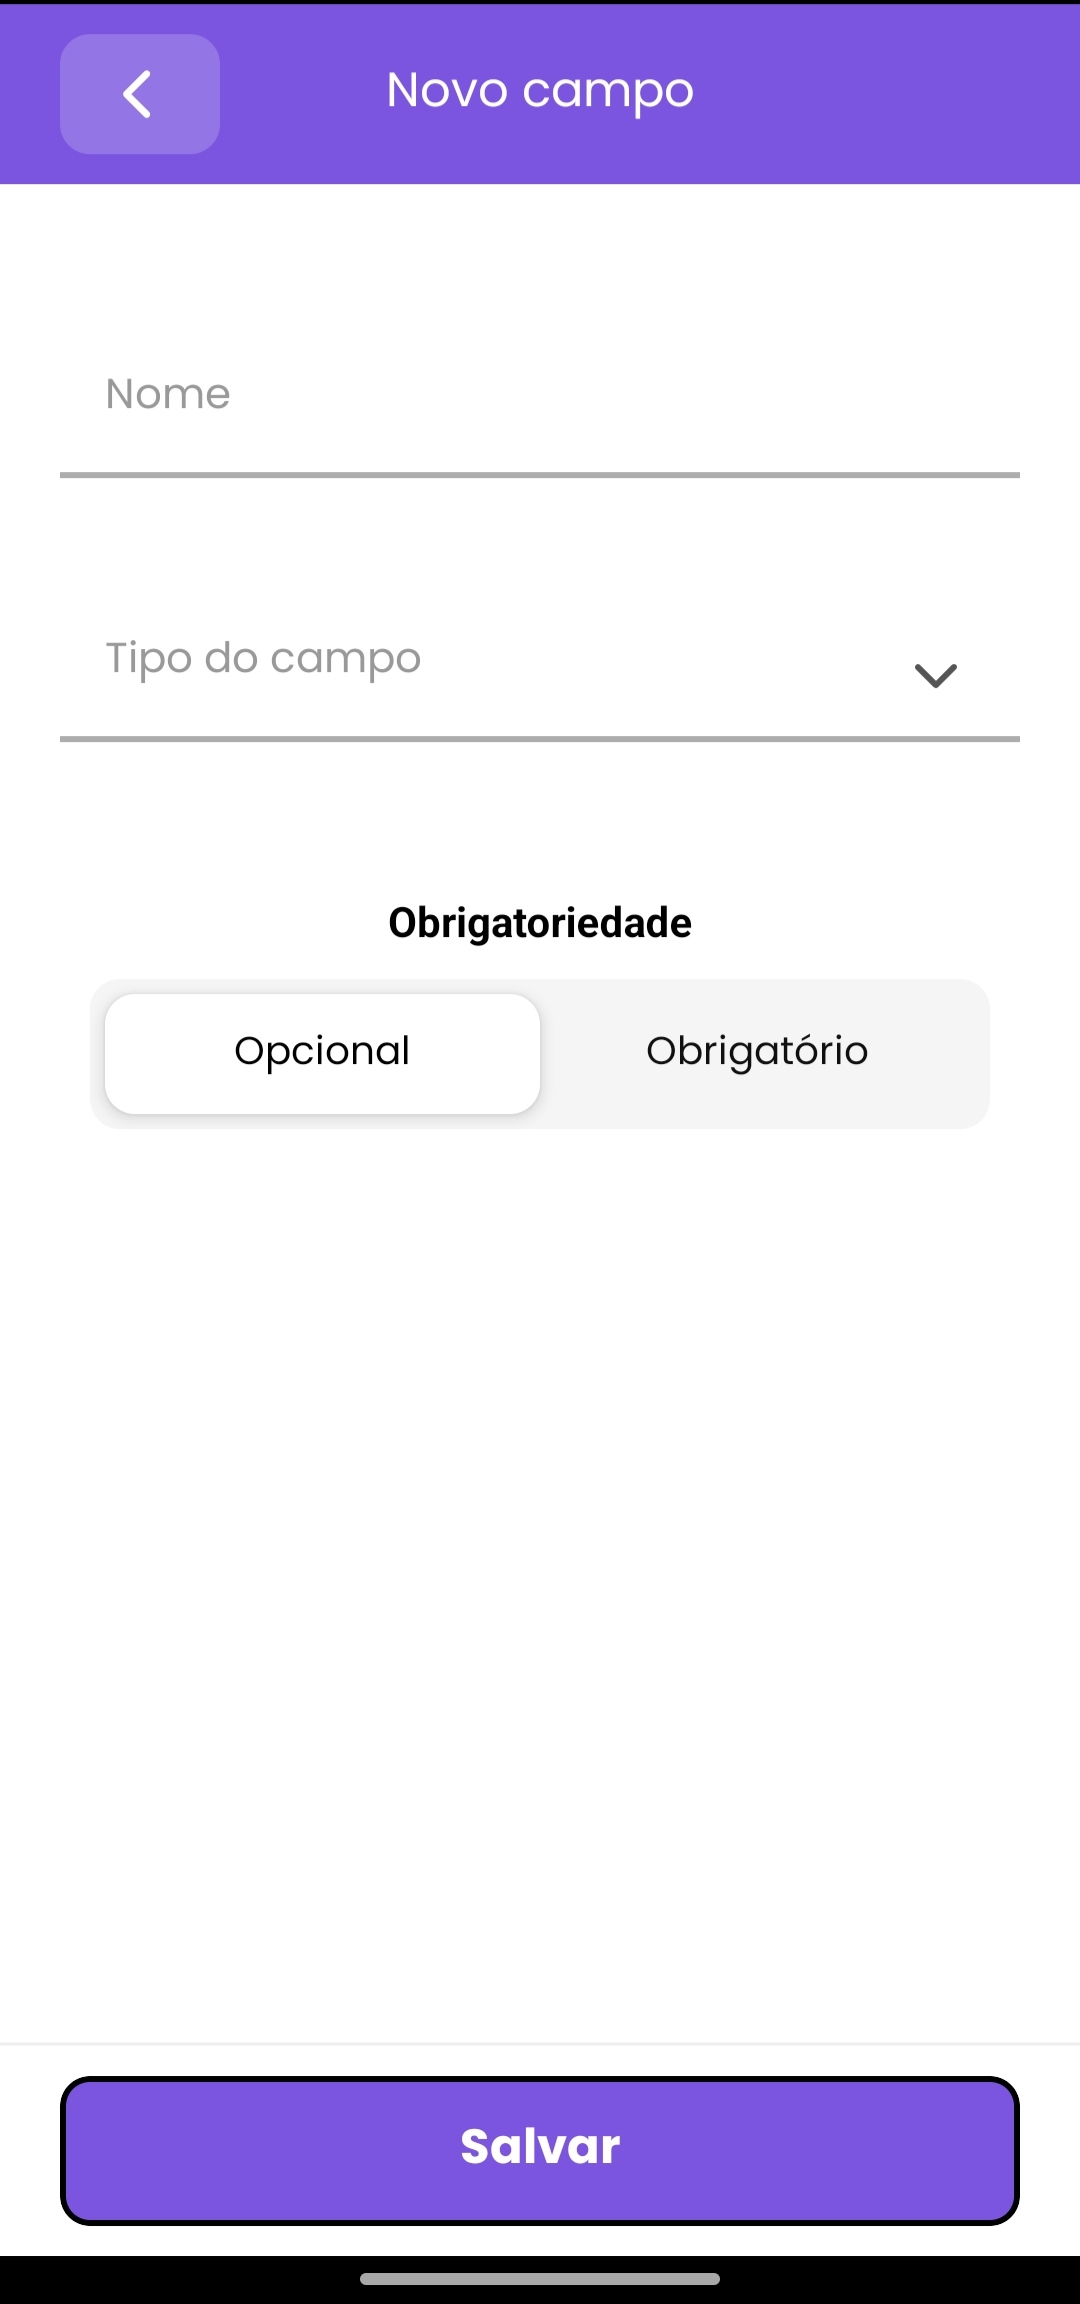
\includegraphics[width=0.45\textwidth,keepaspectratio]{imagens/app/new_dynamic_field.jpg}
    \vspace{0.4cm}
    \end{figure}

Durante a adição de um novo campo, formulários objetivos oferecem escolhas precisas como tipo de dado, obrigatoriedade e máscara, dando total flexibilidade ao criador sem sobrecarregar a experiência visual.

% ───────────────────
\begin{figure}[H]
    \centering
    \caption{Lista de Convidados e Seleção em Massa (\texttt{guestsTab.js})}
    \vspace{0.4cm}
    
\includegraphics[width=0.45\textwidth,keepaspectratio]{imagens/app/list_guests_selection.jpg}
    \vspace{0.4cm}
    \end{figure}

A gestão de convidados foi desenhada para suportar um alto volume de informações com agilidade. Ao manter um toque longo sobre um participante, o organizador ativa o modo de seleção em lote, que transforma o cabeçalho em um painel de ferramentas em massa. Isso possibilita disparar envios de ingressos, certificados ou realizar check-ins múltiplos de uma só vez, otimizando muito o trabalho repetitivo.

% ───────────────────
\begin{figure}[H]
    \centering
    \caption{Lista de Convidados — Visualização Padrão}
    \vspace{0.4cm}
    
\includegraphics[width=0.45\textwidth,keepaspectratio]{imagens/app/list_guests.jpg}
    \vspace{0.4cm}
    \end{figure}

A visualização padrão apresenta indicativos visuais de presença (check-in) em tempo real. Além disso, abas e filtros simplificados permitem isolar convidados por status, auxiliando ativamente o fluxo rápido em recepções e bilheterias físicas.

% ───────────────────
\begin{figure}[H]
    \centering
    \caption{Convidados — Estado Vazio}
    \vspace{0.4cm}
    
\includegraphics[width=0.45\textwidth,keepaspectratio]{imagens/app/empty_guests.jpg}
    \vspace{0.4cm}
    \end{figure}

Novamente, ilustrações contextualizadas apoiam o organizador quando a lista ainda não possui nenhum convidado registrado, preenchendo a tela em branco de forma orgânica.

% ───────────────────
\begin{figure}[H]
    \centering
    \caption{Cadastro Manual de Convidado (\texttt{newGuest.js})}
    \vspace{0.4cm}
    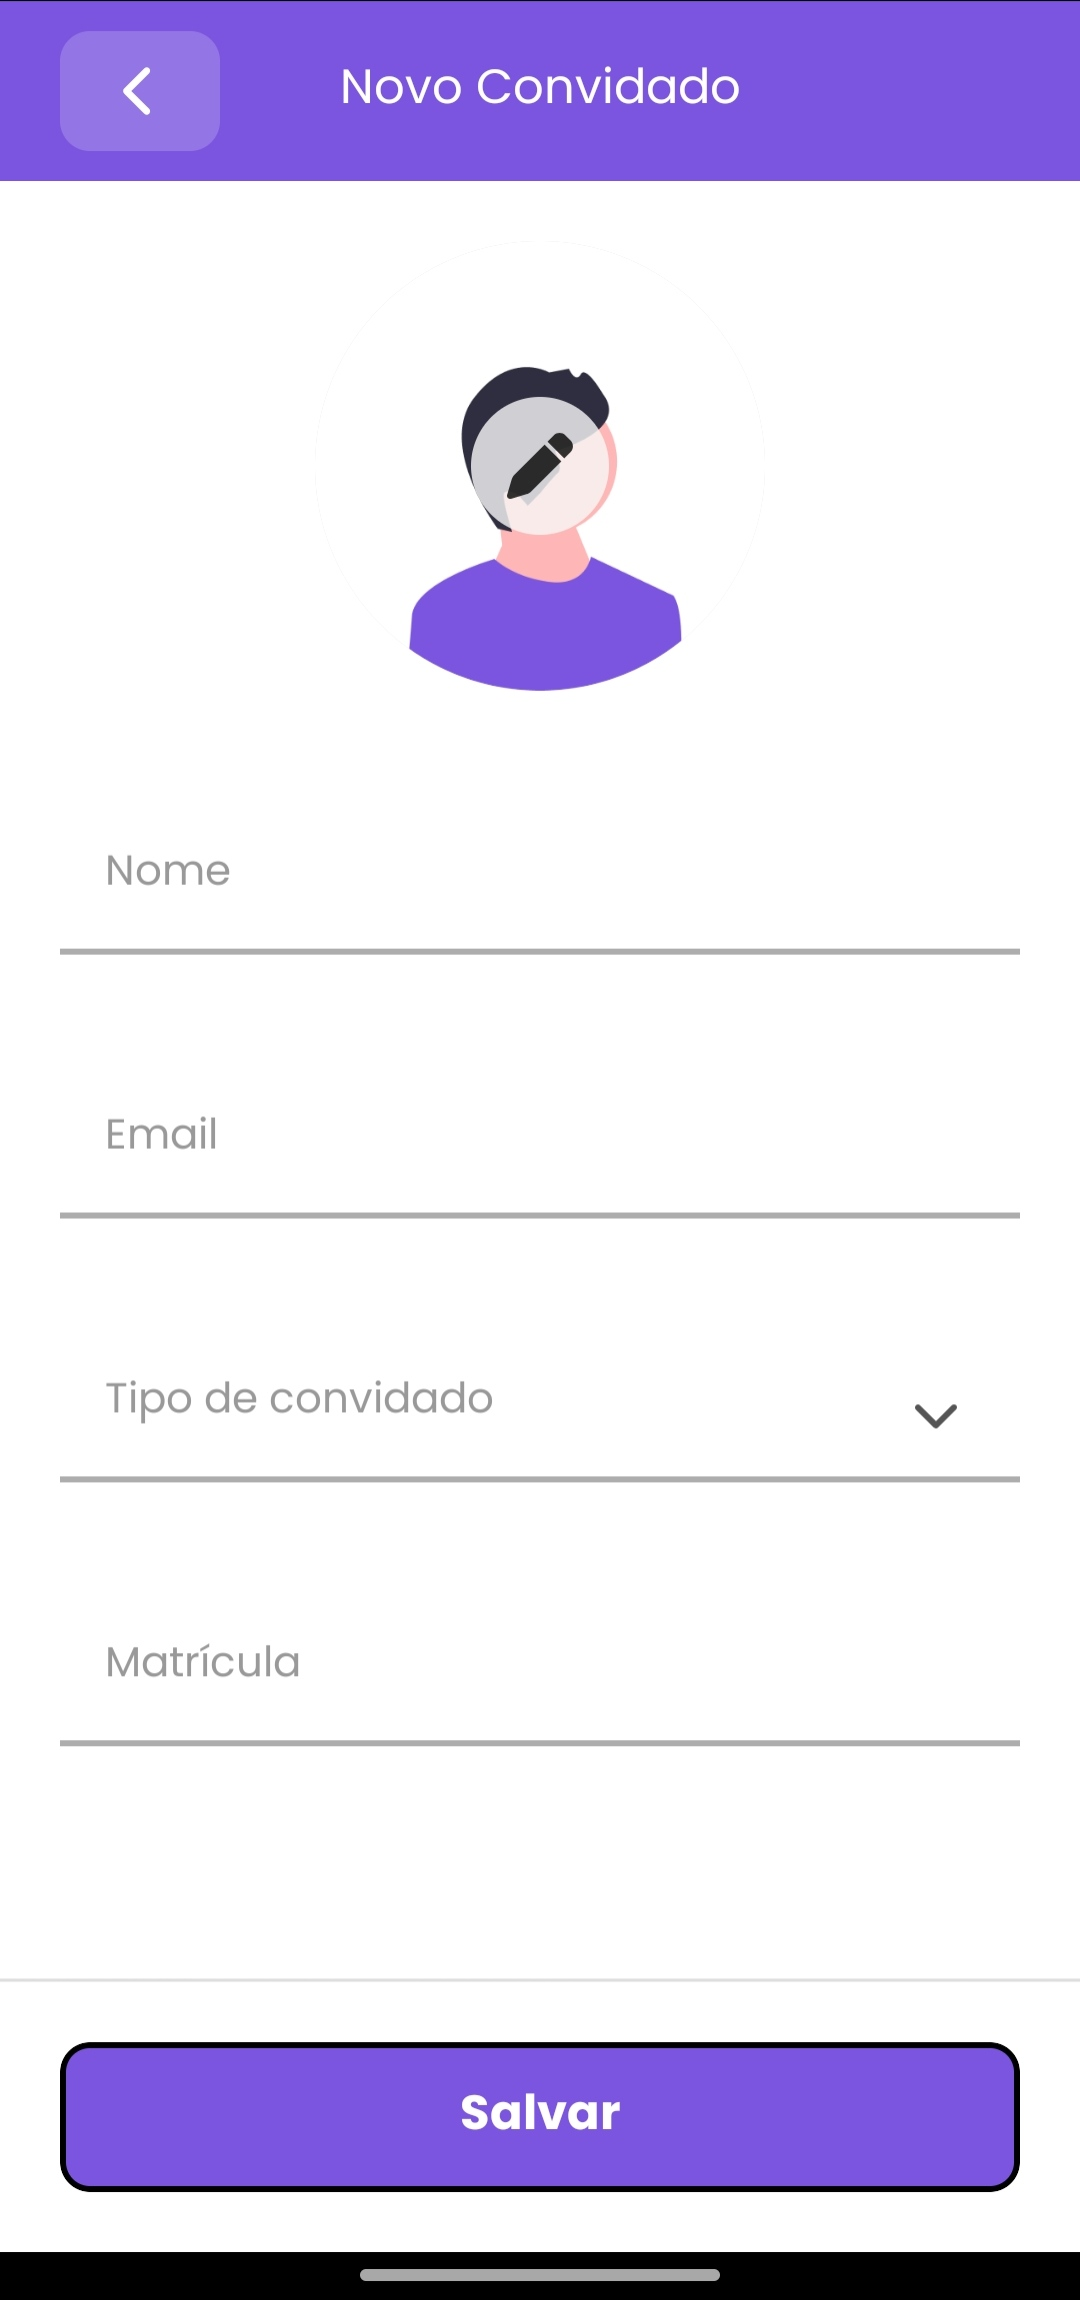
\includegraphics[width=0.45\textwidth,keepaspectratio]{imagens/app/new_guest.jpg}
    \vspace{0.4cm}
    \end{figure}

A interface de cadastro manual é inteiramente adaptável. Baseada nos campos previamente definidos pelo administrador, ela constrói os espaços de preenchimento de forma dinâmica. Dependendo do formato do dado (texto genérico, número, data etc.), o componente visual adequado (teclado numérico ou calendário nativo) se apresenta para evitar falhas de digitação.

% ───────────────────
\begin{figure}[H]
    \centering
    \caption{Detalhes do Convidado (\texttt{guest.js})}
    \vspace{0.4cm}
    
\includegraphics[width=0.45\textwidth,keepaspectratio]{imagens/app/guest_checkin.jpg}
    \vspace{0.4cm}
    \end{figure}

Acessando a página detalhada, há um acompanhamento claro sobre todas as respostas fornecidas pelo participante, encabeçadas por um grande botão em destaque projetado exclusivamente para o controle manual de presença.

% ───────────────────
\begin{figure}[H]
    \centering
    \caption{Opções Adicionais do Convidado}
    \vspace{0.4cm}
    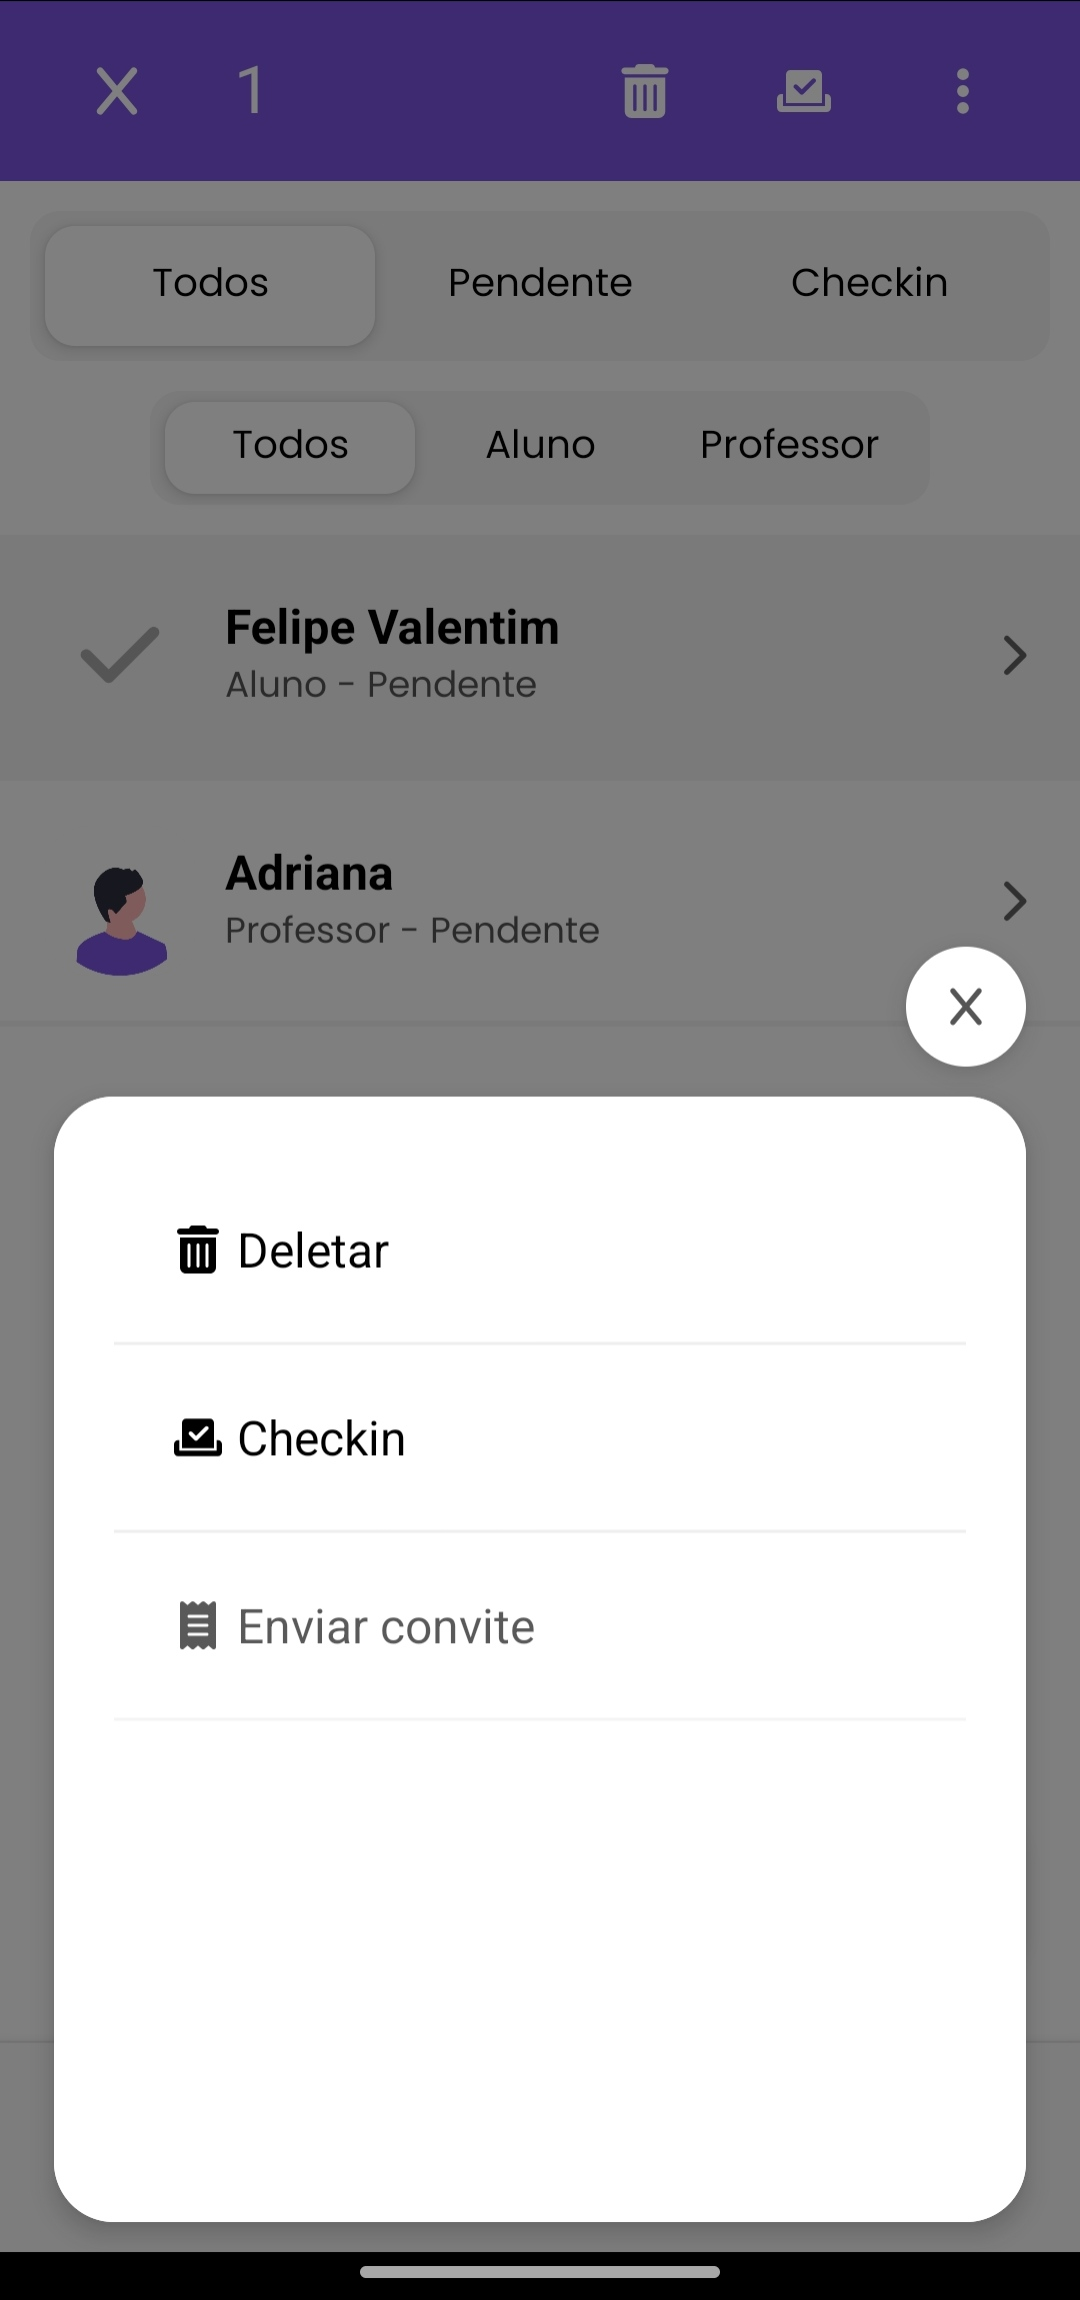
\includegraphics[width=0.45\textwidth,keepaspectratio]{imagens/app/guest_options.jpg}
    \vspace{0.4cm}
    \end{figure}

Para organizar funções extras sem poluir a visão principal, o projeto faz uso de menus e painéis inferiores (\textit{bottom sheets}) flutuantes. Estas áreas acomodam opções mais destrutivas ou esporádicas, como exclusão ou reenvio de convites individualizados.

% ───────────────────
\begin{figure}[H]
    \centering
    \caption{Confirmação de Check-in Manual}
    \vspace{0.4cm}
    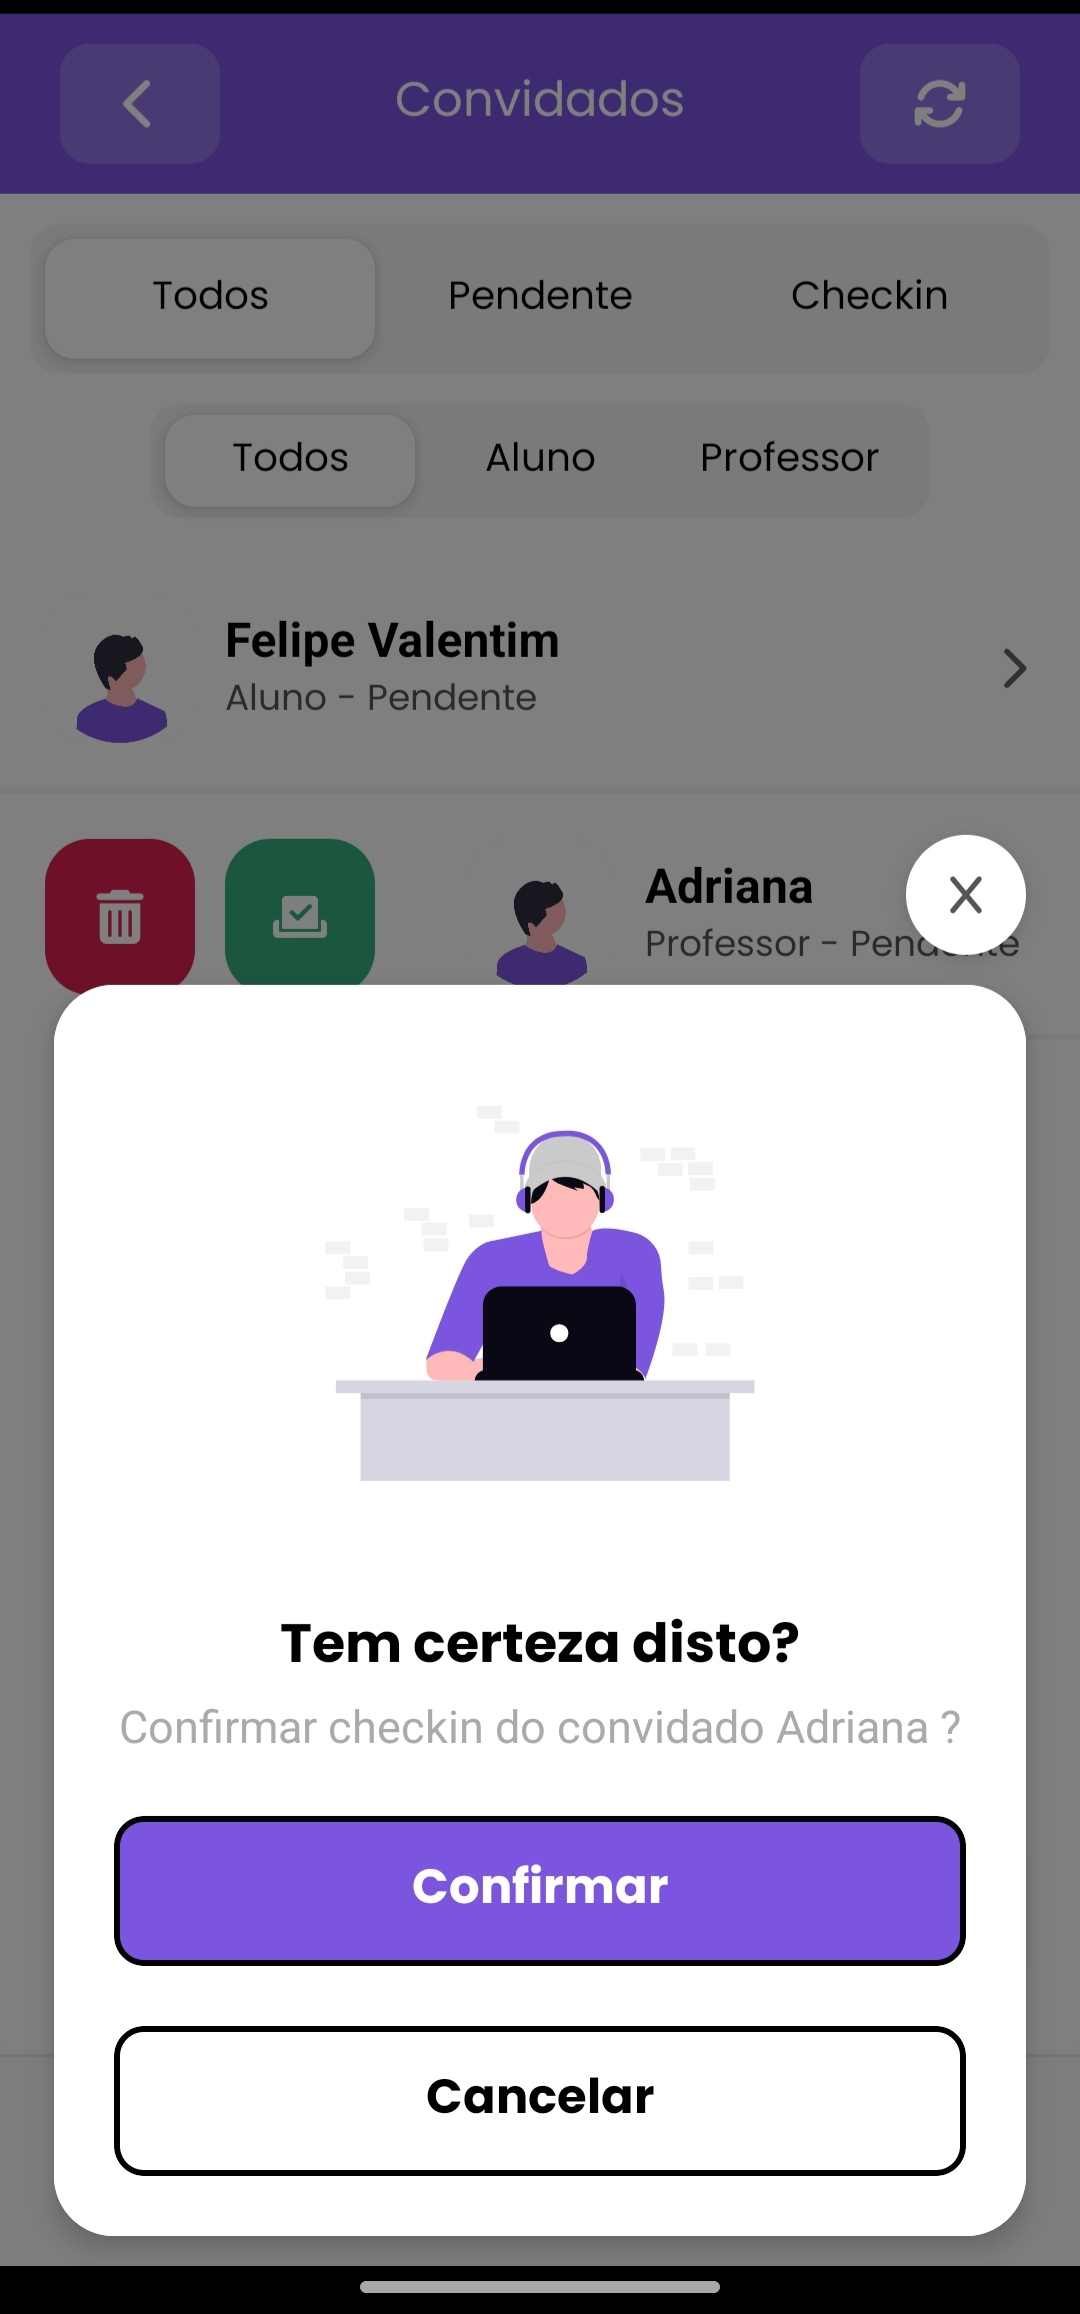
\includegraphics[width=0.45\textwidth,keepaspectratio]{imagens/app/guest_confirm_checkin.jpg}
    \vspace{0.4cm}
    \end{figure}

Ações delicadas, como forçar a entrada ou saída manual de convidados através de botões, acionam pop-ups informativos com linguagem clara, dando total previsibilidade ao organizador sobre o ato.

% ───────────────────
\begin{figure}[H]
    \centering
    \caption{Formulário Público de Auto-Inscrição de Convidados}
    \vspace{0.4cm}
    
\includegraphics[width=0.45\textwidth,keepaspectratio]{imagens/app/guest_registration.jpg}
    \vspace{0.4cm}
    \end{figure}

Expandindo o ecossistema mobile, a interface de auto-inscrição permite que o próprio convidado acesse o formulário web do evento externamente, inserindo seus dados de forma autônoma sem necessidade de conta prévia. A estética desta página age como uma tela de destino (\textit{landing page}) moderna e limpa.

% ───────────────────
\begin{figure}[H]
    \centering
    \caption{Aba de Certificado e Template (\texttt{templateTab.js})}
    \vspace{0.4cm}
    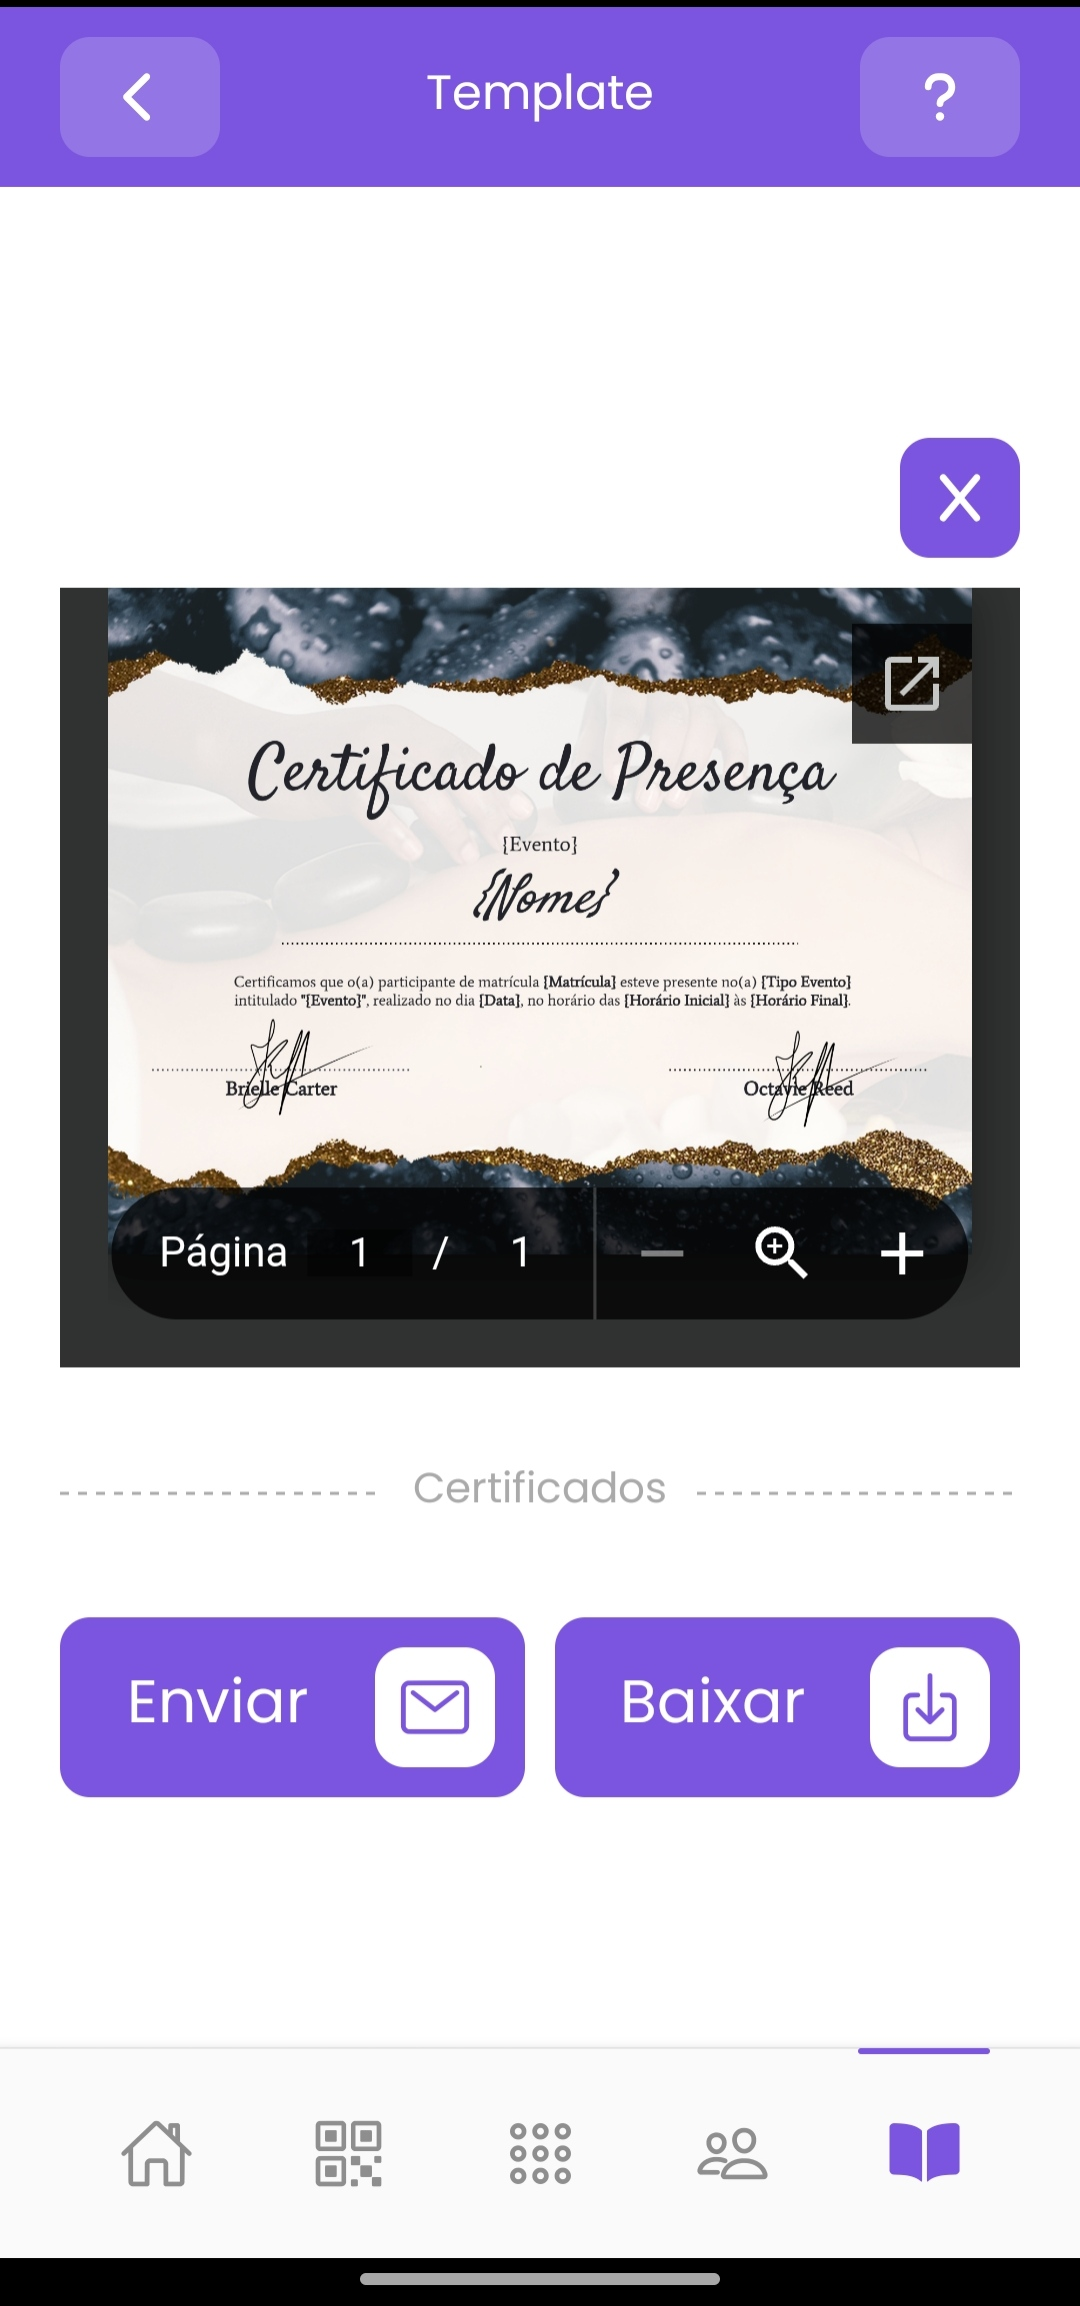
\includegraphics[width=0.45\textwidth,keepaspectratio]{imagens/app/template_preview.jpg}
    \vspace{0.4cm}
    \end{figure}

O gerenciador de certificados propõe uma integração robusta que capacita o organizador a enviar um arquivo formatado (como documento Microsoft Word) para ser usado de espelho. Em seguida, o próprio aplicativo renderiza e exibe visualmente uma miniatura fiel do PDF final, atestando a qualidade do documento antes de envios em massa.

% ───────────────────
\begin{figure}[H]
    \centering
    \caption{Lista de Variáveis (Placeholders) do Template}
    \vspace{0.4cm}
    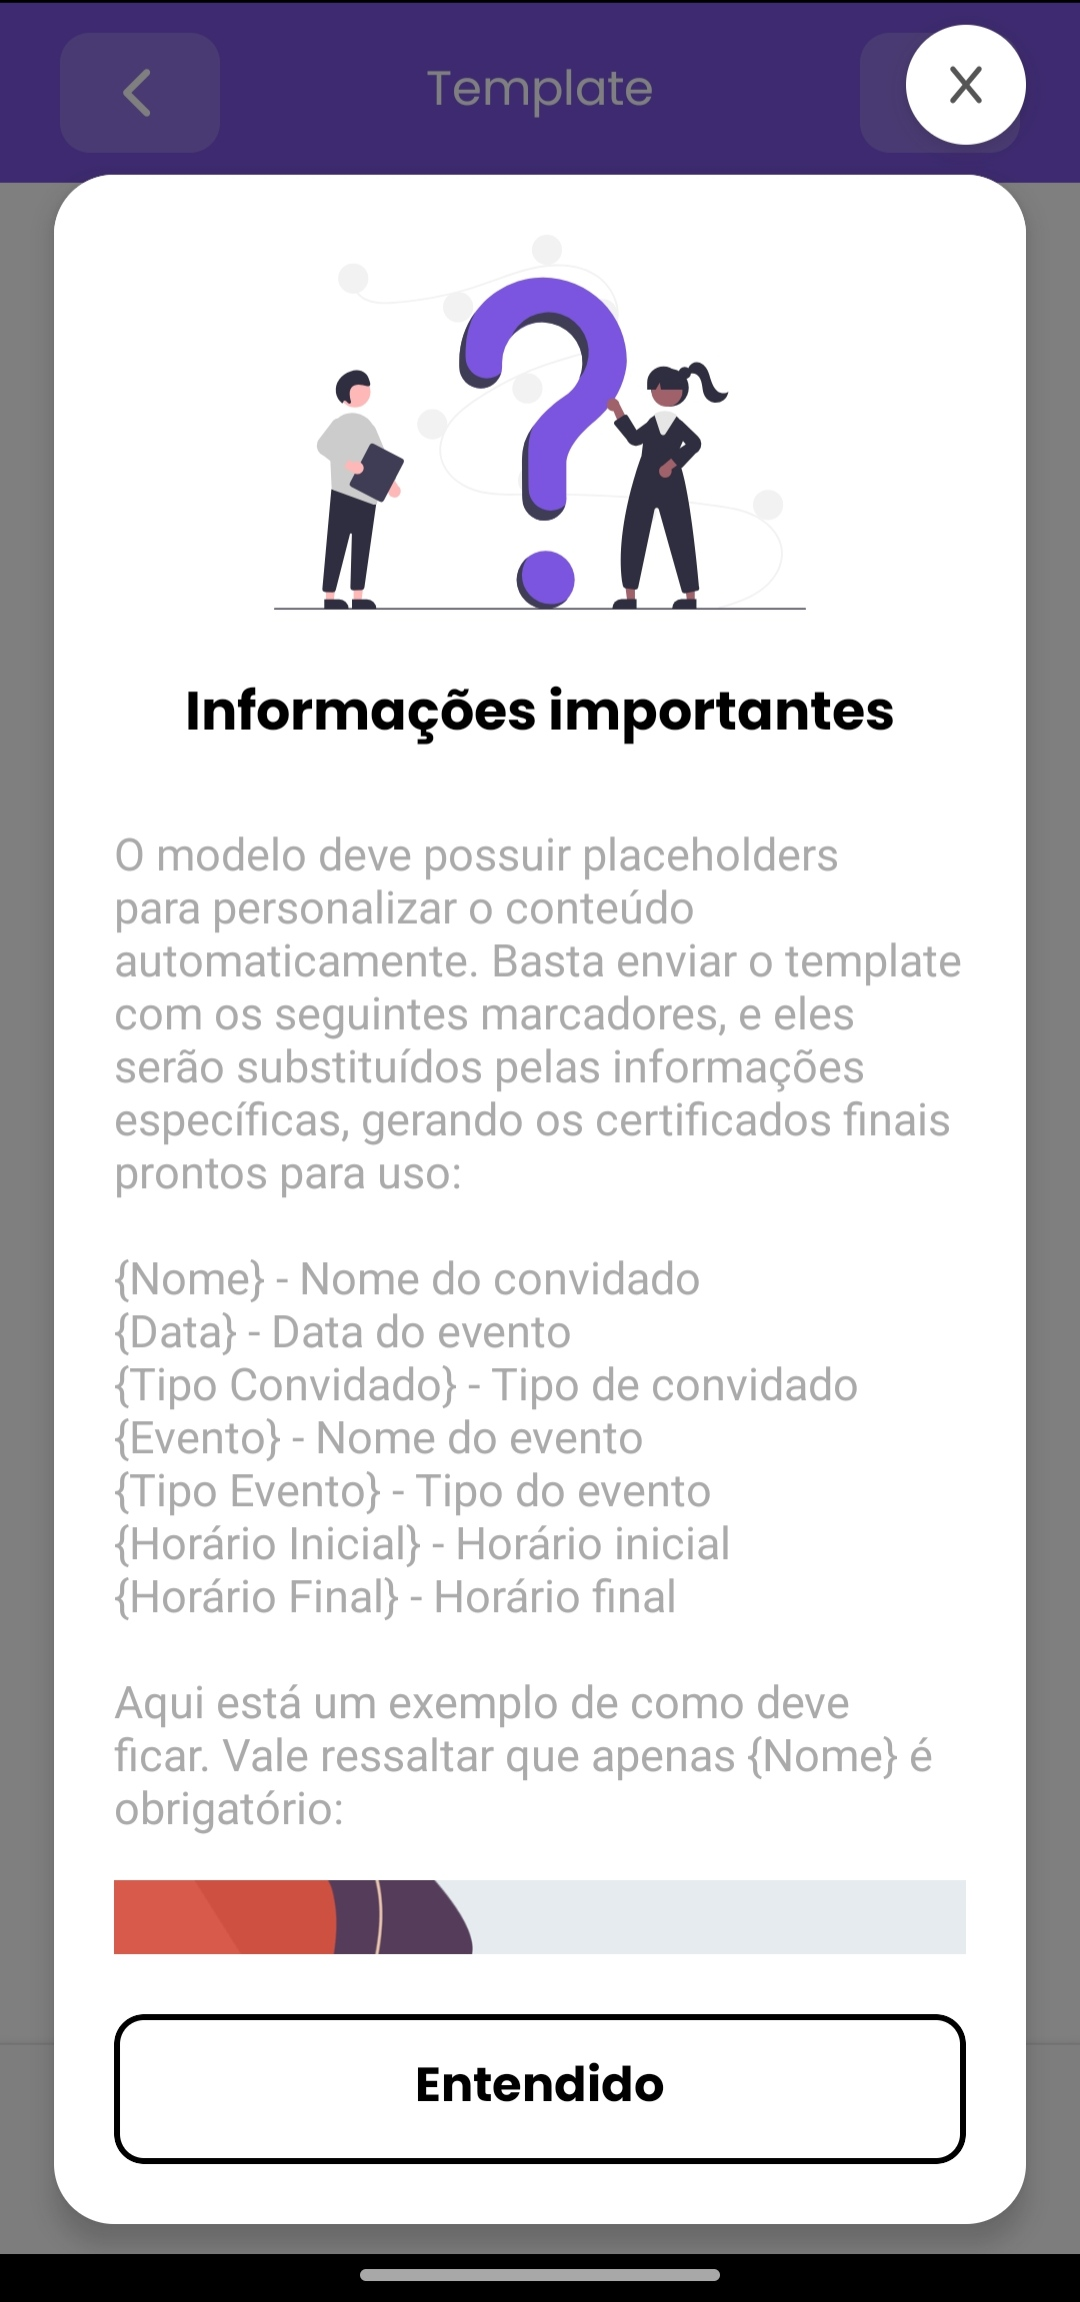
\includegraphics[width=0.45\textwidth,keepaspectratio]{imagens/app/template_placeholders.jpg}
    \vspace{0.4cm}
    \end{figure}

Para mitigar incertezas na confecção do modelo textual, a interface oferece um guia sobreposto com a listagem exata de todas as etiquetas customizadas e variáveis associadas ao evento (\textit{placeholders}). Isso instrui precisamente como a plataforma fará a fusão automatizada dos textos baseando-se nos formulários dos convidados.

% ───────────────────
\begin{figure}[H]
    \centering
    \caption{Confirmação de Exclusão de Template}
    \vspace{0.4cm}
    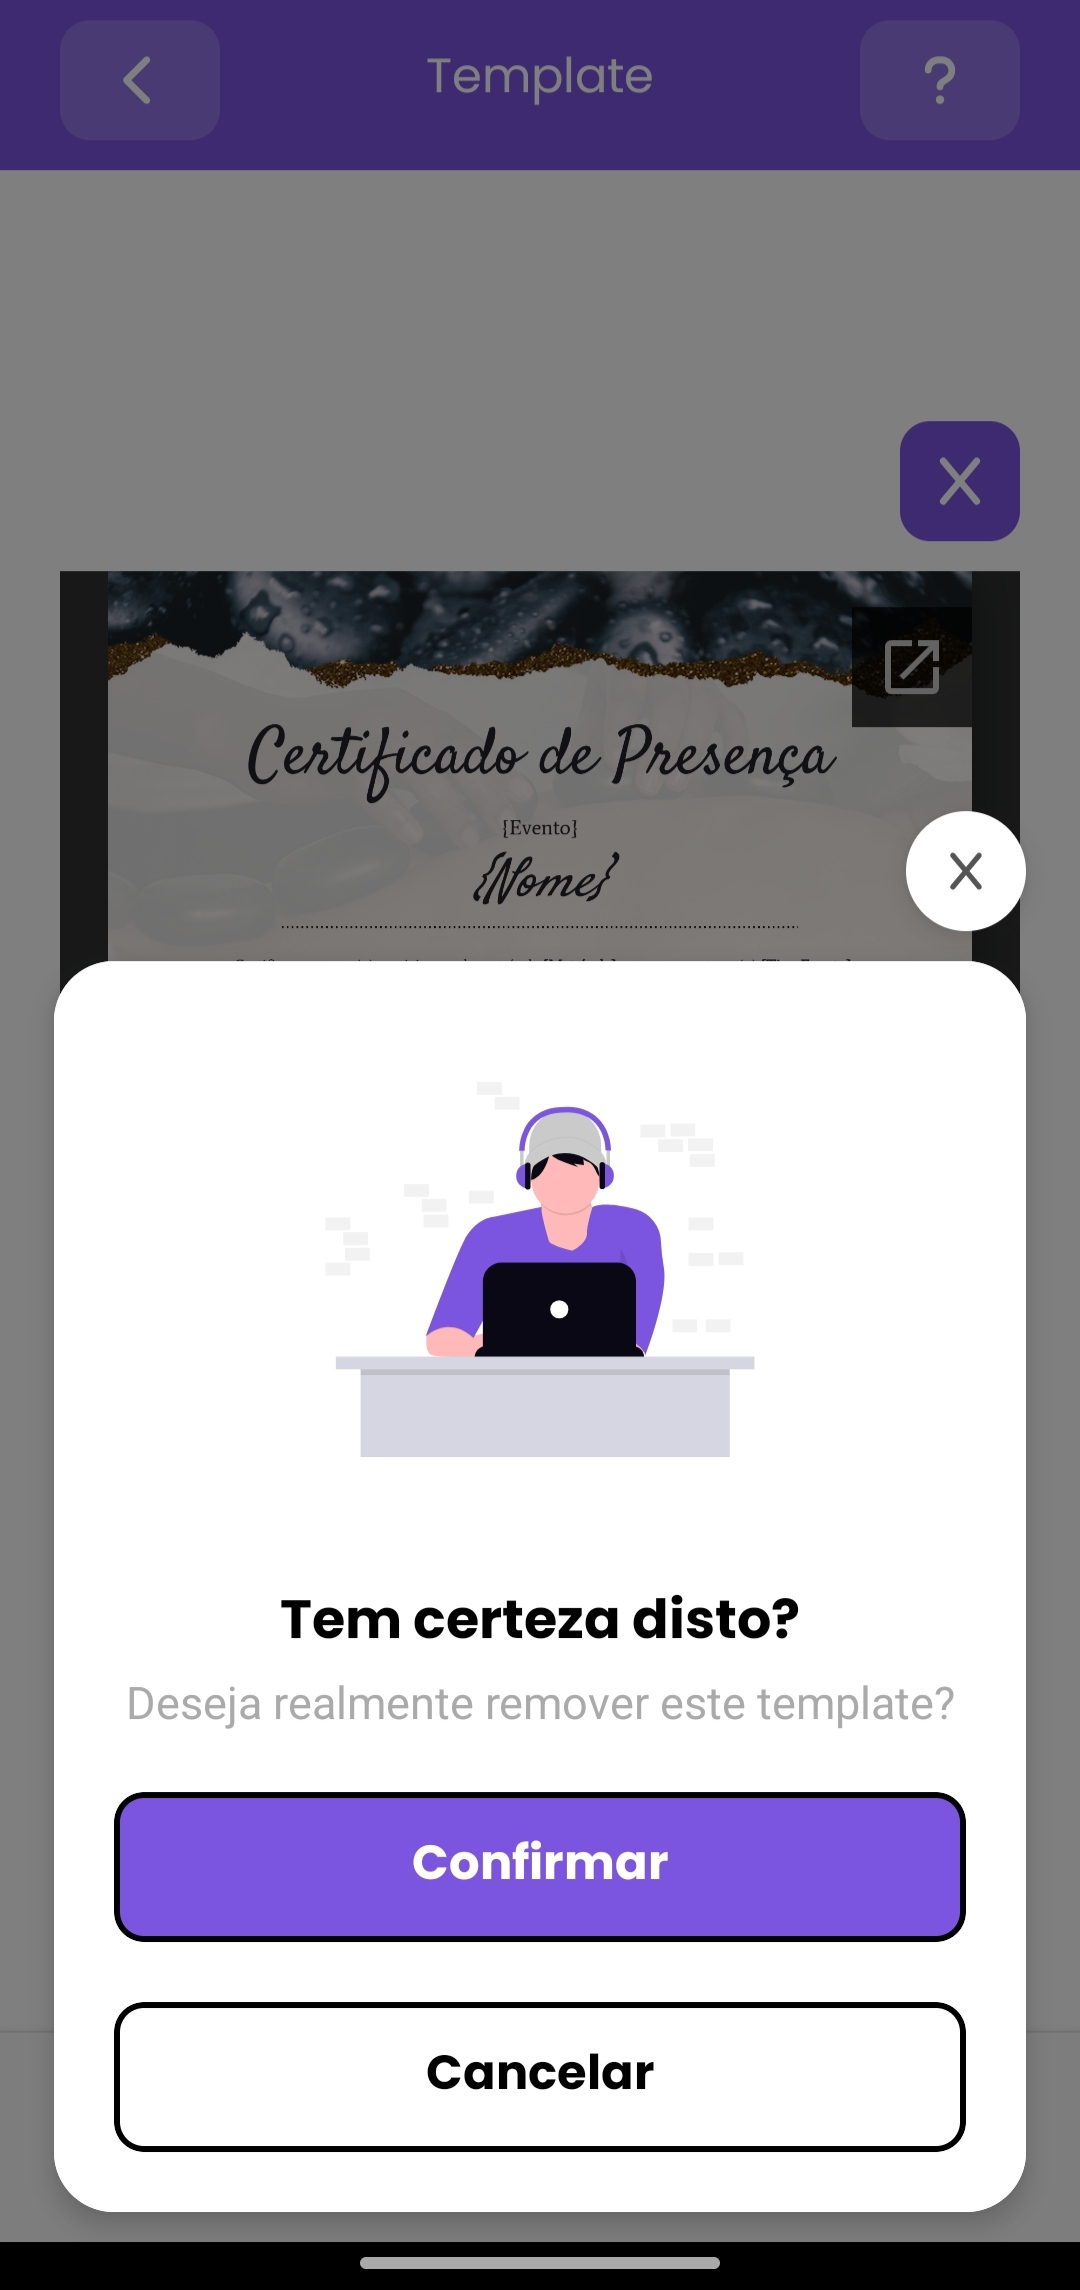
\includegraphics[width=0.45\textwidth,keepaspectratio]{imagens/app/template_confirm_remove.jpg}
    \vspace{0.4cm}
    \end{figure}

Respeitando a heurística constante da plataforma em torno do perdão ao erro, a remoção do documento aciona obrigatoriamente um modal de salvaguarda, conscientizando o usuário da consequência no momento em que se tenta destituir o modelo principal.

% ───────────────────
\begin{figure}[H]
    \centering
    \caption{Templates — Estado Vazio}
    \vspace{0.4cm}
    
\includegraphics[width=0.45\textwidth,keepaspectratio]{imagens/app/empty_templates.jpg}
    \vspace{0.4cm}
    \end{figure}

Quando a plataforma detecta a total ausência de modelos configurados, o aspecto utilitário cede lugar para um estilo receptivo e diretivo, exibindo a funcionalidade inerte junto de um convite acionável evidente para resolver aquela pendência.
